%%%%%%%%%%%%%%%%%%%%%%%%%%%%%%%%%%%%%%%%%
% Beamer Presentation
% LaTeX Template
% Version 1.0 (10/11/12)
%
% This template has been downloaded from:
% http://www.LaTeXTemplates.com
%
% License:
% CC BY-NC-SA 3.0 (http://creativecommons.org/licenses/by-nc-sa/3.0/)
%
%%%%%%%%%%%%%%%%%%%%%%%%%%%%%%%%%%%%%%%%%

%----------------------------------------------------------------------------------------
%	PACKAGES AND THEMES
%----------------------------------------------------------------------------------------

\documentclass{beamer}

\mode<presentation> {

% The Beamer class comes with a number of default slide themes
% which change the colors and layouts of slides. Below this is a list
% of all the themes, uncomment each in turn to see what they look like.

%\usetheme{default}
%\usetheme{AnnArbor}
%\usetheme{Antibes}
%\usetheme{Bergen}
%\usetheme{Berkeley}
%\usetheme{Berlin}
%\usetheme{Boadilla}
%\usetheme{CambridgeUS}
%\usetheme{Copenhagen}
%\usetheme{Darmstadt}
%\usetheme{Dresden}
%\usetheme{Frankfurt}
%\usetheme{Goettingen}
%\usetheme{Hannover}
%\usetheme{Ilmenau}
%\usetheme{JuanLesPins}
%\usetheme{Luebeck}
\usetheme{Madrid}
\usepackage{pbox}
\usepackage{listings}
\lstset{language=Java,
                basicstyle=\footnotesize\ttfamily,
                keywordstyle=\footnotesize\color{blue}\ttfamily,
}

%\usetheme{Malmoe}
%\usetheme{Marburg}
%\usetheme{Montpellier}
%\usetheme{PaloAlto}
%\usetheme{Pittsburgh}
%\usetheme{Rochester}
%\usetheme{Singapore}
%\usetheme{Szeged}
%\usetheme{Warsaw}

% As well as themes, the Beamer class has a number of color themes
% for any slide theme. Uncomment each of these in turn to see how it
% changes the colors of your current slide theme.

%\usecolortheme{albatross}
%\usecolortheme{beaver}
%\usecolortheme{beetle}
%\usecolortheme{crane}
%\usecolortheme{dolphin}
%\usecolortheme{dove}
%\usecolortheme{fly}
%\usecolortheme{lily}
%\usecolortheme{orchid}
%\usecolortheme{rose}
%\usecolortheme{seagull}
%\usecolortheme{seahorse}
%\usecolortheme{whale}
%\usecolortheme{wolverine}

%\setbeamertemplate{footline} % To remove the footer line in all slides uncomment this line
%\setbeamertemplate{footline}[page number] % To replace the footer line in all slides with a simple slide count uncomment this line

%\setbeamertemplate{navigation symbols}{} % To remove the navigation symbols from the bottom of all slides uncomment this line
}

\usepackage{graphicx} % Allows including images
\usepackage{booktabs} % Allows the use of \toprule, \midrule and \bottomrule in tables
\usepackage{framed}

%----------------------------------------------------------------------------------------
%	TITLE PAGE
%----------------------------------------------------------------------------------------

\title[Generici e Collezioni]{Polimorfismo} % The short title appears at the bottom of every slide, the full title is only on the title page

\author{Claudio Menghi} % Your name
\institute[Polimi] % Your institution as it will appear on the bottom of every slide, may be shorthand to save space
{
Politecnico di Milano \\ % Your institution for the title page
\medskip
\textit{claudio.menghi@polimi.it} % Your email address
}
\date{\today} % Date, can be changed to a custom date

\begin{document}

\begin{frame}
\titlepage % Print the title page as the first slide
\end{frame}

\begin{frame}
\frametitle{Overview} % Table of contents slide, comment this block out to remove it
\tableofcontents % Throughout your presentation, if you choose to use \section{} and \subsection{} commands, these will automatically be printed on this slide as an overview of your presentation
\end{frame}

%----------------------------------------------------------------------------------------
%	PRESENTATION SLIDES
%----------------------------------------------------------------------------------------


%------------------------------------------------


\section{Polimorfismo e Binding dinamico}
\subsection{Principio di sostituibilit\`a}

\begin{frame}
\frametitle{Principio di sostituibilit\`a}
\begin{framed}
Il principio di sostituibilit\`a afferma che, se S \`e un sottotipo di T, allora oggetti dichiarati di tipo T possono essere sostituiti con oggetti di tipo S senza alterare la correttezza dei risultati del programma.
\end{framed}
\end{frame}

\begin{frame}[fragile]
\frametitle{Principio di sostituibilit\`a}
\begin{figure}[h!]
  \centering
    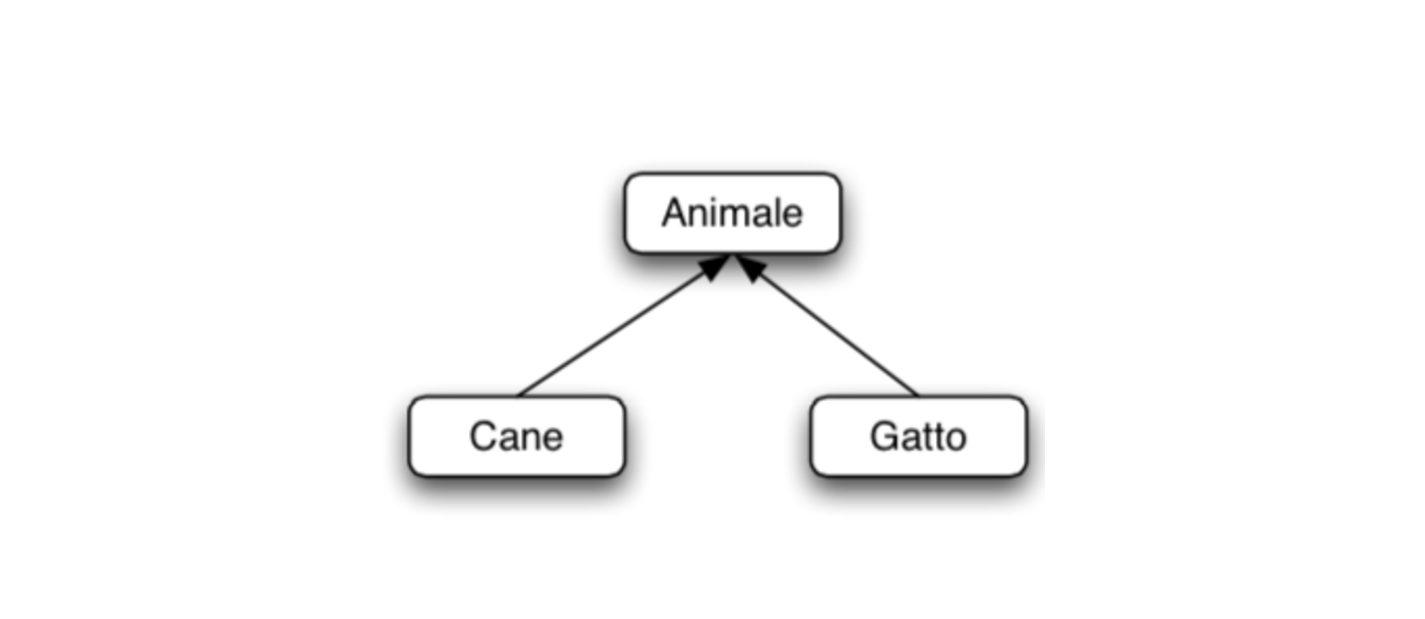
\includegraphics[width=0.7\textwidth]{gerarchia.pdf}
\end{figure}

Quale \`e corretta?
\begin{framed}
\begin{lstlisting}
Animale a=new Cane();
Cane c=new Animale();
\end{lstlisting}
\end{framed}
\end{frame}


\begin{frame}[fragile]
\frametitle{Principio di sostituibilit\`a}
Quale \`e corretta?
\begin{framed}
\begin{lstlisting}
Animale a=new Cane();//ok
Cane c=new Animale(); // errore di compilazione
//Type mismatch: cannot convert from Animale to Cane
\end{lstlisting}
\end{framed}
\end{frame}

\begin{frame}[fragile]
\frametitle{Principio di sostituibilit\`a}
Quale il tipo statico di a? 
\begin{framed}
\begin{lstlisting}
Animale a=new Cane();//ok
\end{lstlisting}
\end{framed}
\end{frame}

\begin{frame}[fragile]
\frametitle{Principio di sostituibilit\`a}
Quale il tipo statico di a? 
\begin{framed}
\begin{lstlisting}
Animale a=new Cane();
// Animale
\end{lstlisting}
\end{framed}
\end{frame}

\begin{frame}[fragile]
\frametitle{Principio di sostituibilit\`a}
Quale il tipo dinamico di a? 
\begin{framed}
\begin{lstlisting}
Animale a=new Cane();
// Cane
\end{lstlisting}
\end{framed}
\end{frame}


\subsection{Overriding}
\begin{frame}[fragile]
\frametitle{Overriding}
\begin{framed}
Overriding:
\begin{itemize}
\item La lista degli argomenti deve essere esattamente la stessa di quella del metodo overridato
\item il tipo di ritorno deve essere lo stesso o un sottotipo di quello del metodo overridato
\item il modificatore di accesso non pu\`o essere pi\`u restrittivo
\item un metodo dichiarato final non pu\`o essere overridato
\item un metodo statico non pu\`o essere overridato ma pu\`o essere ridichiarato
\item constructors cannot be overridden.
\end{itemize}
\end{framed}
\end{frame}


\begin{frame}[fragile]
\frametitle{Overriding}
\begin{framed}
Che cosa stampa?
\begin{lstlisting}
public class Animale {
    public Animale uccidi(Animale altroAnimale){
        System.out.println("Animale: uccidi");
        return altroAnimale;
}}
public class Cane extends Animale {
}
public class Main {
    public static void main(String[] args) {
        Animale b=new Cane();
        Animale a=new Cane();
        a.uccidi(b);
    }
}
\end{lstlisting}
\end{framed}
\end{frame}

\begin{frame}[fragile]
\frametitle{Overriding}
\begin{framed}
Viene stampato Animale: uccidi
\end{framed}
\end{frame}

\begin{frame}[fragile]
\frametitle{Overriding}
\begin{framed}
E' lecito?
\begin{lstlisting}
public class Animale {
    public Animale uccidi(Animale altroAnimale){
        System.out.println("Animale: uccidi");
        return altroAnimale;
}}
public class Cane extends Animale {
}
public class Main {
    public static void main(String[] args) {
        Cane b=new Cane();
        Animale a=new Cane();
        a.uccidi(b);
    }
}
\end{lstlisting}
\end{framed}
\end{frame}

\begin{frame}[fragile]
\frametitle{Overriding}
\begin{framed}
Si la signature \texttt{a.uccidi(b);} \`e consistente con la signature
 \texttt{public Animale uccidi(Animale altroAnimale)}: b \`e di tipo Cane che \`e sottotipo di animale.
\end{framed}
\end{frame}

\begin{frame}[fragile]
\frametitle{Overriding}
\begin{framed}
Che cosa stampa?
\begin{lstlisting}
public class Animale {
    public Animale uccidi(Animale altroAnimale){
        System.out.println("Animale: uccidi");
        return altroAnimale;
}}
public class Cane extends Animale {
    public Animale uccidi(Cane altroAnimale){
        System.out.println("Cane: uccidi");
        return altroAnimale;
}}
public class Main {
    public static void main(String[] args) {
        Cane b=new Cane();
        Animale a=new Cane();
        a.uccidi(b);
    }
}
\end{lstlisting}
\end{framed}
\end{frame}

\begin{frame}[fragile]
\frametitle{Overriding}
\begin{framed}
Animale: uccidi
\end{framed}
\end{frame}

\begin{frame}[fragile]
\frametitle{Overriding}
\begin{framed}
Che cosa stampa?
\begin{lstlisting}
public class Animale {
	public Animale uccidi(Animale altroAnimale){
	    System.out.println("Animale: uccidi");
	    return altroAnimale;
}}
public class Cane extends Animale {
	public Animale uccidi(Cane altroAnimale){
	    System.out.println("Cane: uccidi");
	    return altroAnimale;
}}
public class Main {
    public static void main(String[] args) {
        Cane b=new Cane();
        Animale a=new Cane();
        b.uccidi(a);
   }
}
\end{lstlisting}
\end{framed}
\end{frame}

\begin{frame}[fragile]
\frametitle{Overriding}
\begin{framed}
Animale: uccidi
\end{framed}
\end{frame}


\begin{frame}[fragile]
\frametitle{Overriding}
\begin{framed}
Che cosa stampa?
\begin{lstlisting}
public class Animale {
    public Animale uccidi(Animale altroAnimale){
        System.out.println("Animale: uccidi");
        return altroAnimale;
}}
public class Cane extends Animale {
    public Animale uccidi(Cane altroAnimale){
        System.out.println("Cane: uccidi");
        return altroAnimale;
}}
public class Main {
    public static void main(String[] args) {
        Cane b=new Cane();
        Animale a=new Cane();
        b.uccidi(b);
   }
}
\end{lstlisting}
\end{framed}
\end{frame}

\begin{frame}[fragile]
\frametitle{Overriding}
\begin{framed}
Cane: uccidi
\end{framed}
\end{frame}


\begin{frame}[fragile]
\begin{columns}
\begin{column}{0.6\textwidth}
\begin{lstlisting}[language=Java,escapechar=|]
public class ClassA {
    public void stampa(ClassA p){
        System.out.println("AAA");
    }
}
\end{lstlisting}
\begin{lstlisting}[language=Java,escapechar=|]
public class ClassB extends ClassA {
    public void stampa(ClassB p){
        System.out.println("BBB");
    }
    public void stampa(ClassA p){
        System.out.println("AAA/BBB");
    }
}
\end{lstlisting}
\begin{lstlisting}[language=Java,escapechar=|]
public class ClassC extends ClassA {
    public void stampa(ClassC p){
        System.out.println("CCC");
    }
    public void stampa(ClassA p){
        System.out.println("AAA/CCC");
   }
}
\end{lstlisting}
\end{column}
\begin{column}{0.4\textwidth}
\begin{lstlisting}[language=Java,escapechar=|]
public static void main(
    String[] args) {
    ClassA a1, a2;
    ClassB b1;
    ClassC c1;
    a1 = new ClassB();
    b1 = new ClassB();
    c1 = new ClassC();
    a2 = new ClassC();
    b1.stampa(b1); 
   
}
\end{lstlisting}
\end{column}
\end{columns}
\end{frame}

\begin{frame}[fragile]
\begin{columns}
\begin{column}{0.6\textwidth}
\begin{lstlisting}[language=Java,escapechar=|]
public class ClassA {
    public void stampa(ClassA p){
        System.out.println("AAA");
    }
}
\end{lstlisting}
\begin{lstlisting}[language=Java,escapechar=|]
public class ClassB extends ClassA {
    public void stampa(ClassB p){
        System.out.println("BBB");
    }
    public void stampa(ClassA p){
        System.out.println("AAA/BBB");
    }
}
\end{lstlisting}
\begin{lstlisting}[language=Java,escapechar=|]
public class ClassC extends ClassA {
    public void stampa(ClassC p){
        System.out.println("CCC");
    }
    public void stampa(ClassA p){
        System.out.println("AAA/CCC");
   }
}
\end{lstlisting}
\end{column}
\begin{column}{0.4\textwidth}
\begin{lstlisting}[language=Java,escapechar=|]
public static void main(
    String[] args) {
    ClassA a1, a2;
    ClassB b1;
    ClassC c1;
    a1 = new ClassB();
    b1 = new ClassB();
    c1 = new ClassC();
    a2 = new ClassC();
    b1.stampa(b1); 
    // BBB
}
\end{lstlisting}
\end{column}
\end{columns}
\end{frame}


\begin{frame}[fragile]
\begin{columns}
\begin{column}{0.6\textwidth}
\begin{lstlisting}[language=Java,escapechar=|]
public class ClassA {
    public void stampa(ClassA p){
        System.out.println("AAA");
    }
}
\end{lstlisting}
\begin{lstlisting}[language=Java,escapechar=|]
public class ClassB extends ClassA {
    public void stampa(ClassB p){
        System.out.println("BBB");
    }
    public void stampa(ClassA p){
        System.out.println("AAA/BBB");
    }
}
\end{lstlisting}
\begin{lstlisting}[language=Java,escapechar=|]
public class ClassC extends ClassA {
    public void stampa(ClassC p){
        System.out.println("CCC");
    }
    public void stampa(ClassA p){
        System.out.println("AAA/CCC");
   }
}
\end{lstlisting}
\end{column}
\begin{column}{0.4\textwidth}
\begin{lstlisting}[language=Java,escapechar=|]
public static void main(
    String[] args) {
    ClassA a1, a2;
    ClassB b1;
    ClassC c1;
    a1 = new ClassB();
    b1 = new ClassB();
    c1 = new ClassC();
    a2 = new ClassC();
    b1.stampa(b1); 
    // BBB
    a1.stampa(b1); 
}
\end{lstlisting}
\end{column}
\end{columns}
\end{frame}


\begin{frame}[fragile]
\begin{columns}
\begin{column}{0.6\textwidth}
\begin{lstlisting}[language=Java,escapechar=|]
public class ClassA {
    public void stampa(ClassA p){
        System.out.println("AAA");
    }
}
\end{lstlisting}
\begin{lstlisting}[language=Java,escapechar=|]
public class ClassB extends ClassA {
    public void stampa(ClassB p){
        System.out.println("BBB");
    }
    public void stampa(ClassA p){
        System.out.println("AAA/BBB");
    }
}
\end{lstlisting}
\begin{lstlisting}[language=Java,escapechar=|]
public class ClassC extends ClassA {
    public void stampa(ClassC p){
        System.out.println("CCC");
    }
    public void stampa(ClassA p){
        System.out.println("AAA/CCC");
   }
}
\end{lstlisting}
\end{column}
\begin{column}{0.4\textwidth}
\begin{lstlisting}[language=Java,escapechar=|]
public static void main(
    String[] args) {
    ClassA a1, a2;
    ClassB b1;
    ClassC c1;
    a1 = new ClassB();
    b1 = new ClassB();
    c1 = new ClassC();
    a2 = new ClassC();
    b1.stampa(b1); 
    //BBB
    a1.stampa(b1);  
    //AAA/BBB
}
\end{lstlisting}
\end{column}
\end{columns}
\end{frame}

\begin{frame}[fragile]
\begin{columns}
\begin{column}{0.6\textwidth}
\begin{lstlisting}[language=Java,escapechar=|]
public class ClassA {
    public void stampa(ClassA p){
        System.out.println("AAA");
    }
}
\end{lstlisting}
\begin{lstlisting}[language=Java,escapechar=|]
public class ClassB extends ClassA {
    public void stampa(ClassB p){
        System.out.println("BBB");
    }
    public void stampa(ClassA p){
        System.out.println("AAA/BBB");
    }
}
\end{lstlisting}
\begin{lstlisting}[language=Java,escapechar=|]
public class ClassC extends ClassA {
    public void stampa(ClassC p){
        System.out.println("CCC");
    }
    public void stampa(ClassA p){
        System.out.println("AAA/CCC");
   }
}
\end{lstlisting}
\end{column}
\begin{column}{0.4\textwidth}
\begin{lstlisting}[language=Java,escapechar=|]
public static void main(
    String[] args) {
    ClassA a1, a2;
    ClassB b1;
    ClassC c1;
    a1 = new ClassB();
    b1 = new ClassB();
    c1 = new ClassC();
    a2 = new ClassC();
    b1.stampa(b1); 
    //BBB
    a1.stampa(b1);  
    //AAA/BBB
    b1.stampa(c1);
}
\end{lstlisting}
\end{column}
\end{columns}
\end{frame}

\begin{frame}[fragile]
\begin{columns}
\begin{column}{0.6\textwidth}
\begin{lstlisting}[language=Java,escapechar=|]
public class ClassA {
    public void stampa(ClassA p){
        System.out.println("AAA");
    }
}
\end{lstlisting}
\begin{lstlisting}[language=Java,escapechar=|]
public class ClassB extends ClassA {
    public void stampa(ClassB p){
        System.out.println("BBB");
    }
    public void stampa(ClassA p){
        System.out.println("AAA/BBB");
    }
}
\end{lstlisting}
\begin{lstlisting}[language=Java,escapechar=|]
public class ClassC extends ClassA {
    public void stampa(ClassC p){
        System.out.println("CCC");
    }
    public void stampa(ClassA p){
        System.out.println("AAA/CCC");
   }
}
\end{lstlisting}
\end{column}
\begin{column}{0.4\textwidth}
\begin{lstlisting}[language=Java,escapechar=|]
public static void main(
    String[] args) {
    ClassA a1, a2;
    ClassB b1;
    ClassC c1;
    a1 = new ClassB();
    b1 = new ClassB();
    c1 = new ClassC();
    a2 = new ClassC();
    b1.stampa(b1); 
    //BBB
    a1.stampa(b1);  
    //AAA/BBB
    b1.stampa(c1); 
    // AAA/BBB
}
\end{lstlisting}
\end{column}
\end{columns}
\end{frame}

\begin{frame}[fragile]
\begin{columns}
\begin{column}{0.6\textwidth}
\begin{lstlisting}[language=Java,escapechar=|]
public class ClassA {
    public void stampa(ClassA p){
        System.out.println("AAA");
    }
}
\end{lstlisting}
\begin{lstlisting}[language=Java,escapechar=|]
public class ClassB extends ClassA {
    public void stampa(ClassB p){
        System.out.println("BBB");
    }
    public void stampa(ClassA p){
        System.out.println("AAA/BBB");
    }
}
\end{lstlisting}
\begin{lstlisting}[language=Java,escapechar=|]
public class ClassC extends ClassA {
    public void stampa(ClassC p){
        System.out.println("CCC");
    }
    public void stampa(ClassA p){
        System.out.println("AAA/CCC");
   }
}
\end{lstlisting}
\end{column}
\begin{column}{0.4\textwidth}
\begin{lstlisting}[language=Java,escapechar=|]
public static void main(
    String[] args) {
    ClassA a1, a2;
    ClassB b1;
    ClassC c1;
    a1 = new ClassB();
    b1 = new ClassB();
    c1 = new ClassC();
    a2 = new ClassC();
    b1.stampa(b1); 
    //BBB
    a1.stampa(b1);  
    //AAA/BBB
    b1.stampa(c1); 
    // AAA/BBB
    c1.stampa(c1); 
}
\end{lstlisting}
\end{column}
\end{columns}
\end{frame}

\begin{frame}[fragile]
\begin{columns}
\begin{column}{0.6\textwidth}
\begin{lstlisting}[language=Java,escapechar=|]
public class ClassA {
    public void stampa(ClassA p){
        System.out.println("AAA");
    }
}
\end{lstlisting}
\begin{lstlisting}[language=Java,escapechar=|]
public class ClassB extends ClassA {
    public void stampa(ClassB p){
        System.out.println("BBB");
    }
    public void stampa(ClassA p){
        System.out.println("AAA/BBB");
    }
}
\end{lstlisting}
\begin{lstlisting}[language=Java,escapechar=|]
public class ClassC extends ClassA {
    public void stampa(ClassC p){
        System.out.println("CCC");
    }
    public void stampa(ClassA p){
        System.out.println("AAA/CCC");
   }
}
\end{lstlisting}
\end{column}
\begin{column}{0.4\textwidth}
\begin{lstlisting}[language=Java,escapechar=|]
public static void main(
    String[] args) {
    ClassA a1, a2;
    ClassB b1;
    ClassC c1;
    a1 = new ClassB();
    b1 = new ClassB();
    c1 = new ClassC();
    a2 = new ClassC();
    b1.stampa(b1); 
    //BBB
    a1.stampa(b1);  
    //AAA/BBB
    b1.stampa(c1); 
    // AAA/BBB
    c1.stampa(c1); 
    // CCC
}
\end{lstlisting}
\end{column}
\end{columns}
\end{frame}

\begin{frame}[fragile]
\begin{columns}
\begin{column}{0.6\textwidth}
\begin{lstlisting}[language=Java,escapechar=|]
public class ClassA {
    public void stampa(ClassA p){
        System.out.println("AAA");
    }
}
\end{lstlisting}
\begin{lstlisting}[language=Java,escapechar=|]
public class ClassB extends ClassA {
    public void stampa(ClassB p){
        System.out.println("BBB");
    }
    public void stampa(ClassA p){
        System.out.println("AAA/BBB");
    }
}
\end{lstlisting}
\begin{lstlisting}[language=Java,escapechar=|]
public class ClassC extends ClassA {
    public void stampa(ClassC p){
        System.out.println("CCC");
    }
    public void stampa(ClassA p){
        System.out.println("AAA/CCC");
   }
}
\end{lstlisting}
\end{column}
\begin{column}{0.4\textwidth}
\begin{lstlisting}[language=Java,escapechar=|]
public static void main(
    String[] args) {
    ClassA a1, a2;
    ClassB b1;
    ClassC c1;
    a1 = new ClassB();
    b1 = new ClassB();
    c1 = new ClassC();
    a2 = new ClassC();
    b1.stampa(b1); 
    //BBB
    a1.stampa(b1);  
    //AAA/BBB
    b1.stampa(c1); 
    // AAA/BBB
    c1.stampa(c1); 
    // CCC
    c1.stampa(a1); 
}
\end{lstlisting}
\end{column}
\end{columns}
\end{frame}

\begin{frame}[fragile]
\begin{columns}
\begin{column}{0.6\textwidth}
\begin{lstlisting}[language=Java,escapechar=|]
public class ClassA {
    public void stampa(ClassA p){
        System.out.println("AAA");
    }
}
\end{lstlisting}
\begin{lstlisting}[language=Java,escapechar=|]
public class ClassB extends ClassA {
    public void stampa(ClassB p){
        System.out.println("BBB");
    }
    public void stampa(ClassA p){
        System.out.println("AAA/BBB");
    }
}
\end{lstlisting}
\begin{lstlisting}[language=Java,escapechar=|]
public class ClassC extends ClassA {
    public void stampa(ClassC p){
        System.out.println("CCC");
    }
    public void stampa(ClassA p){
        System.out.println("AAA/CCC");
   }
}
\end{lstlisting}
\end{column}
\begin{column}{0.4\textwidth}
\begin{lstlisting}[language=Java,escapechar=|]
public static void main(
    String[] args) {
    ClassA a1, a2;
    ClassB b1;
    ClassC c1;
    a1 = new ClassB();
    b1 = new ClassB();
    c1 = new ClassC();
    a2 = new ClassC();
    b1.stampa(b1); 
    //BBB
    a1.stampa(b1);  
    //AAA/BBB
    b1.stampa(c1); 
    // AAA/BBB
    c1.stampa(c1); 
    // CCC
    c1.stampa(a1); 
    // AAA/CCC
}
\end{lstlisting}
\end{column}
\end{columns}
\end{frame}


\begin{frame}[fragile]
\begin{columns}
\begin{column}{0.6\textwidth}
\begin{lstlisting}[language=Java,escapechar=|]
public class ClassA {
    public void stampa(ClassA p){
        System.out.println("AAA");
    }
}
\end{lstlisting}
\begin{lstlisting}[language=Java,escapechar=|]
public class ClassB extends ClassA {
    public void stampa(ClassB p){
        System.out.println("BBB");
    }
    public void stampa(ClassA p){
        System.out.println("AAA/BBB");
    }
}
\end{lstlisting}
\begin{lstlisting}[language=Java,escapechar=|]
public class ClassC extends ClassA {
    public void stampa(ClassC p){
        System.out.println("CCC");
    }
    public void stampa(ClassA p){
        System.out.println("AAA/CCC");
   }
}
\end{lstlisting}
\end{column}
\begin{column}{0.4\textwidth}
\begin{lstlisting}[language=Java,escapechar=|]
public static void main(
    String[] args) {
    ClassA a1, a2;
    ClassB b1;
    ClassC c1;
    a1 = new ClassB();
    b1 = new ClassB();
    c1 = new ClassC();
    a2 = new ClassC();
    b1.stampa(b1); 
    //BBB
    a1.stampa(b1);  
    //AAA/BBB
    b1.stampa(c1); 
    // AAA/BBB
    c1.stampa(c1); 
    // CCC
    c1.stampa(a1); 
    // AAA/CCC
     a2.stampa(c1)
}
\end{lstlisting}
\end{column}
\end{columns}
\end{frame}


\begin{frame}[fragile]
\begin{columns}
\begin{column}{0.6\textwidth}
\begin{lstlisting}[language=Java,escapechar=|]
public class ClassA {
    public void stampa(ClassA p){
        System.out.println("AAA");
    }
}
\end{lstlisting}
\begin{lstlisting}[language=Java,escapechar=|]
public class ClassB extends ClassA {
    public void stampa(ClassB p){
        System.out.println("BBB");
    }
    public void stampa(ClassA p){
        System.out.println("AAA/BBB");
    }
}
\end{lstlisting}
\begin{lstlisting}[language=Java,escapechar=|]
public class ClassC extends ClassA {
    public void stampa(ClassC p){
        System.out.println("CCC");
    }
    public void stampa(ClassA p){
        System.out.println("AAA/CCC");
   }
}
\end{lstlisting}
\end{column}
\begin{column}{0.4\textwidth}
\begin{lstlisting}[language=Java,escapechar=|]
public static void main(
    String[] args) {
    ClassA a1, a2;
    ClassB b1;
    ClassC c1;
    a1 = new ClassB();
    b1 = new ClassB();
    c1 = new ClassC();
    a2 = new ClassC();
    b1.stampa(b1); 
    //BBB
    a1.stampa(b1);  
    //AAA/BBB
    b1.stampa(c1); 
    // AAA/BBB
    c1.stampa(c1); 
    // CCC
    c1.stampa(a1); 
    // AAA/CCC
     a2.stampa(c1) 
     // AAA/CCC
}
\end{lstlisting}
\end{column}
\end{columns}
\end{frame}





\section{Interfacce}
\begin{frame}[fragile]
\frametitle{Interfacce}
\begin{figure}[h!]
  \centering
    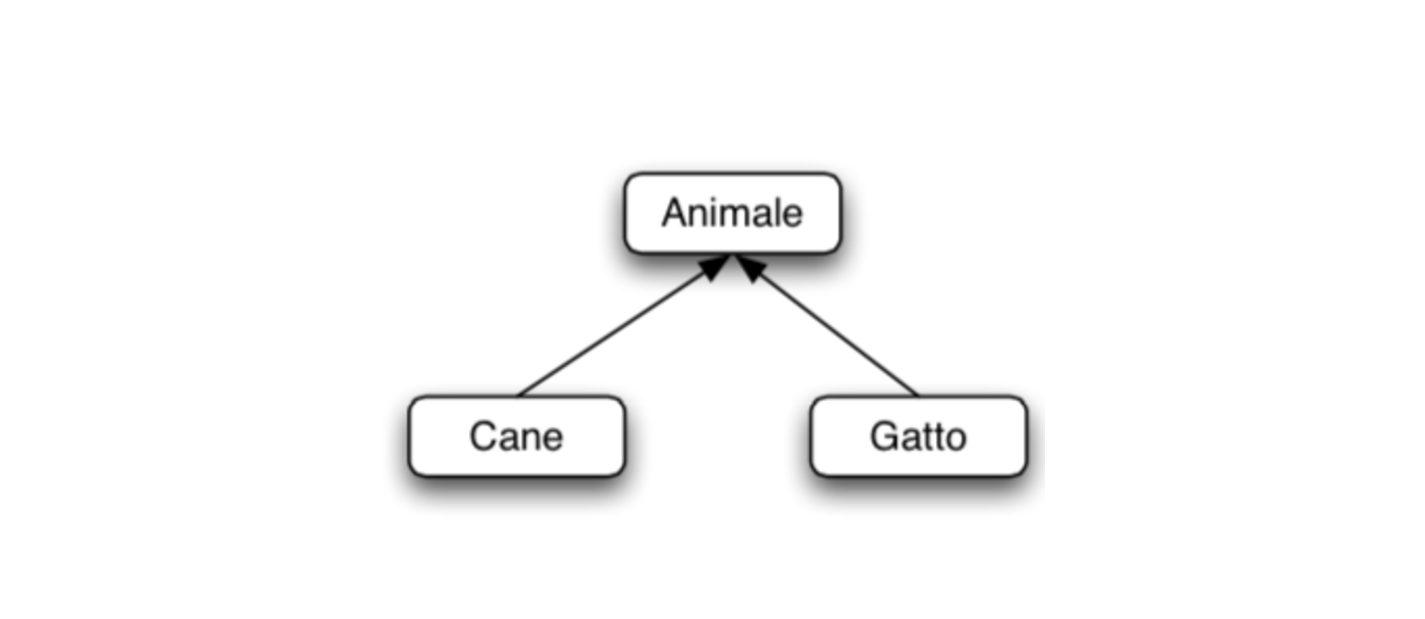
\includegraphics[width=0.7\textwidth]{gerarchia.pdf}
\end{figure}
Vogliamo aggiungere gli animali che sanno volare
\end{frame}

\begin{frame}[fragile]
\frametitle{Interfacce}
\begin{figure}[h!]
  \centering
    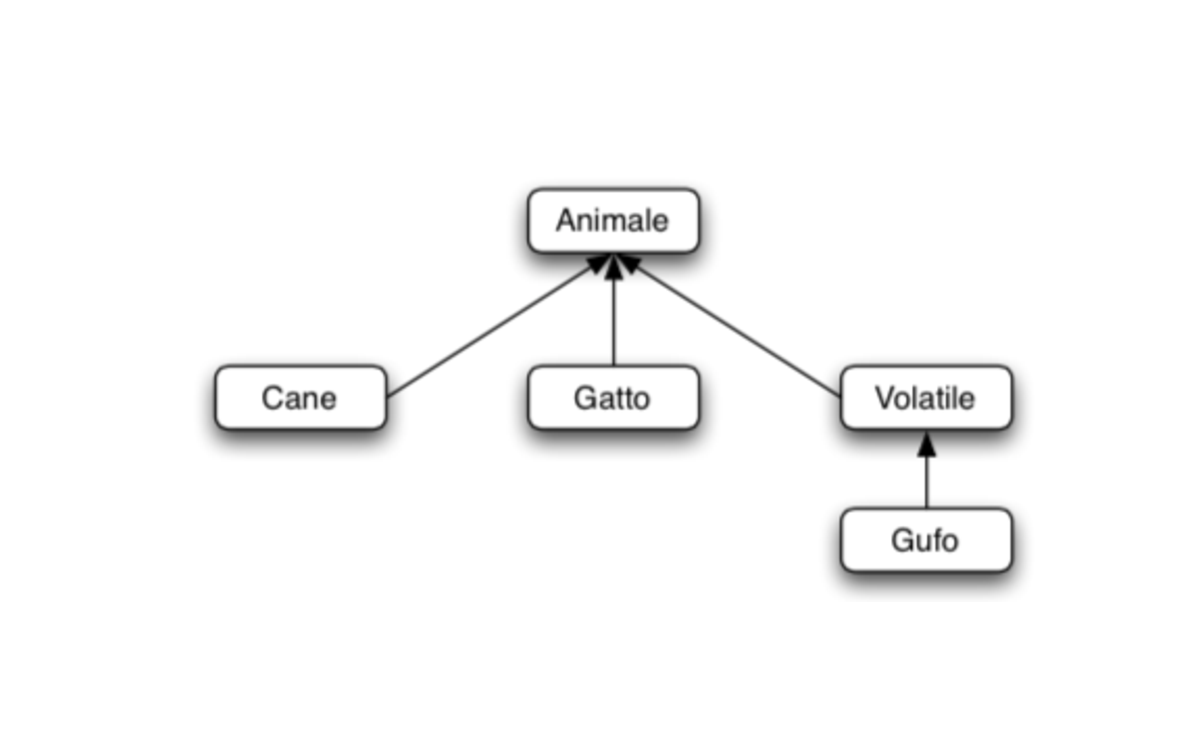
\includegraphics[width=0.7\textwidth]{gerarchia2.pdf}
\end{figure}
Vogliamo aggiungere gli animali che sanno nuotare
\end{frame}


\begin{frame}[fragile]
\frametitle{Interfacce}
\begin{figure}[h!]
  \centering
    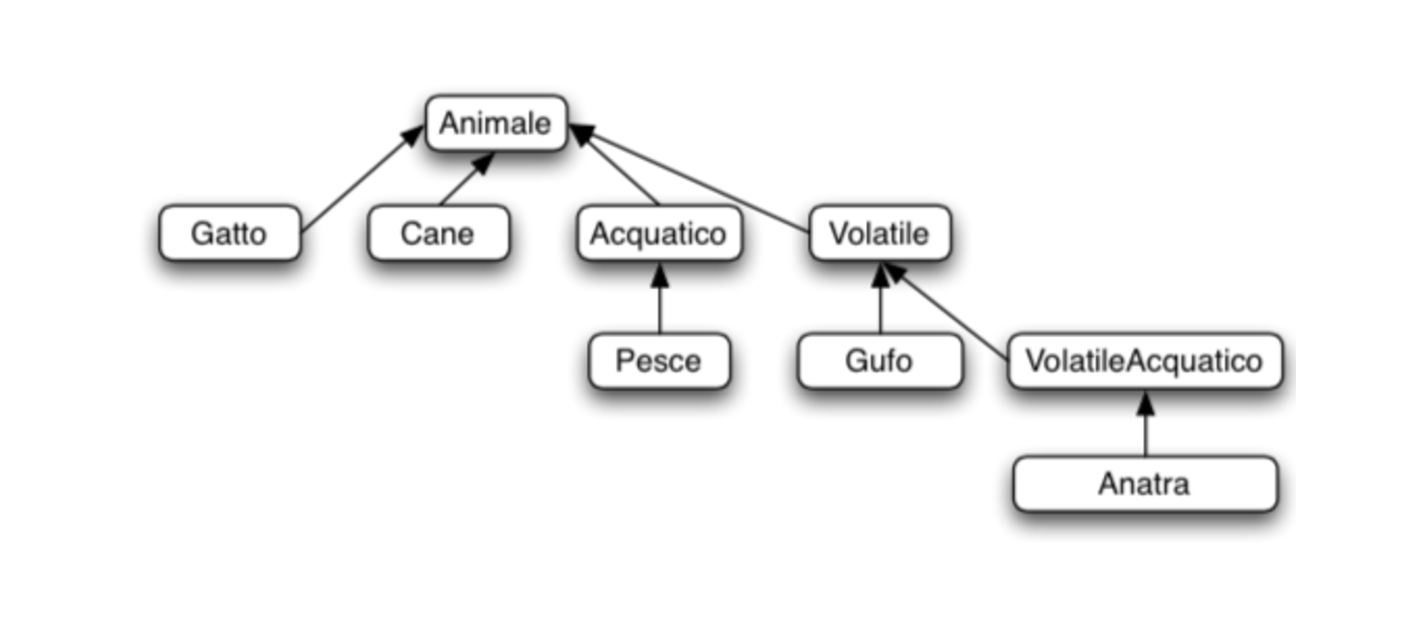
\includegraphics[width=0.7\textwidth]{gerarchia3.pdf}
\end{figure}
\begin{itemize}
\item  piccole modifiche comporano modifiche rilevanti
\item Non dice che pesce e anatra sono entrambi acquatici
\end{itemize}
\end{frame}

\begin{frame}[fragile]
\frametitle{Interfacce}
Per ottenere il risultato sperato ci serve l'ereditariet\`a multipla. In Java l'ereditariet\`a multipla \`e supportata per mezzo delle interfacce
\begin{itemize}
\item  piccole modifiche comporano modifiche rilevanti
\item Non dice che pesce e anatra sono entrambi acquatici
\end{itemize}
\end{frame}

\begin{frame}[fragile]
\frametitle{Interfacce}
\begin{figure}[h!]
  \centering
    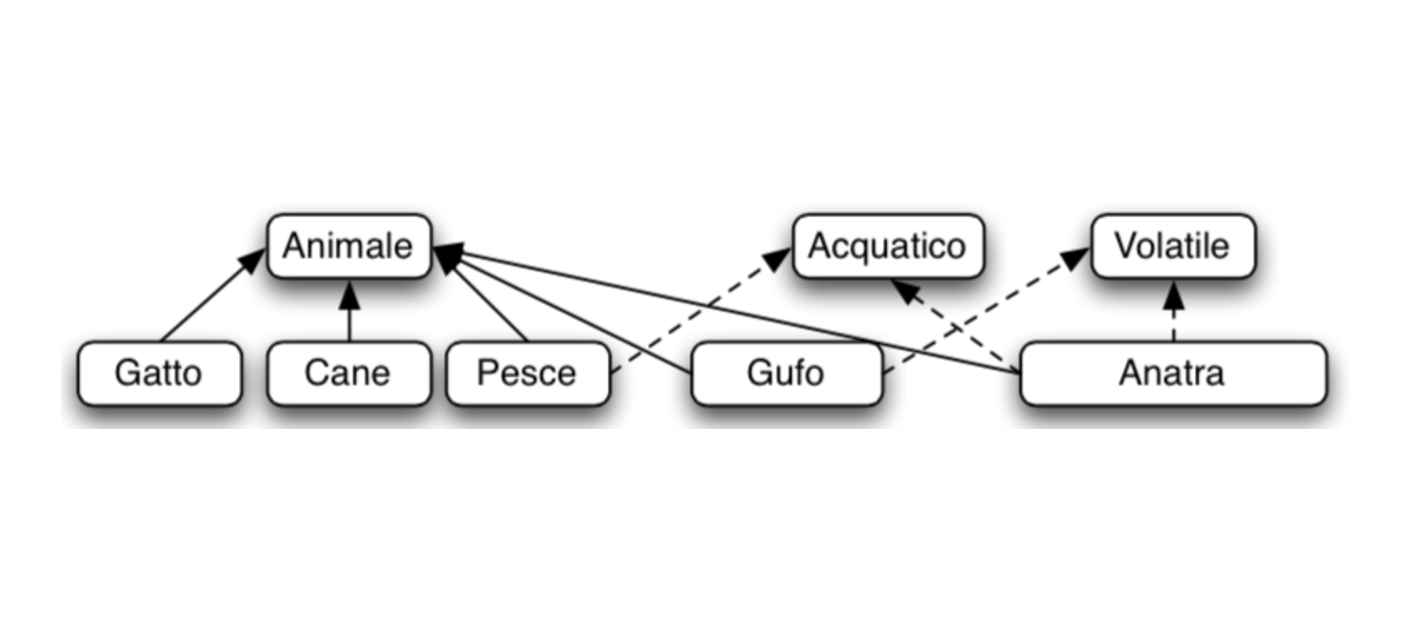
\includegraphics[width=0.7\textwidth]{gerarchia4.pdf}
\end{figure}
\begin{itemize}
\item vantaggi:
\begin{itemize}
\item gerarchia pi\`u semplice
\item possiamo specificare i concetti che ci servono
\end{itemize}
\end{itemize}
\end{frame}

\begin{frame}[fragile]
\frametitle{Interfacce}
\begin{lstlisting}[language=Java,escapechar=|]
public class Anatra extends Animale
     implements Volatile, Acquatico { 
     // Ha tutto ciò che aveva la classe Animale
    // Deve implementare i metodi definiti in 
    // Volatile e in Acquatico 
    @Override
    public void vola(){ ... }
    @Override    
    public void nuota(){ ... } 
}
\end{lstlisting}
\end{frame}

\begin{frame}[fragile]
\frametitle{Interfacce}
 \begin{itemize}
 \item Anche le interfacce possono essere usate come tipo di un riferimento
 \item Come tipo statico, un'interfaccia espone tutti i metodi che definisce
 \item L'implementazione utilizzata dipende dal tipo dinamico della classe (Binding dinamico)
 \item Per gli assegnamenti dobbiamo considerare le relazioni di tipo/sotto-tipo
 \end{itemize}
\end{frame}

\begin{frame}[fragile]
\frametitle{Interfacce}
Quali operazioni sono valide?
\begin{lstlisting}[language=Java,escapechar=|]
Animale g = new Gatto(); 
Pesce p = new Pesce(); 
Anatra a = new Anatra(); 
Volatile g1 = g; 
Volatile v = a;
Nuotatore n = a;
g.vola();
g.nuota();
v.vola();
n.nuota();
\end{lstlisting}
\end{frame}

\begin{frame}[fragile]
\frametitle{Interfacce}
Quali operazioni sono valide?
\begin{lstlisting}[language=Java,escapechar=|]
Animale g = new Gatto(); 
Pesce p = new Pesce(); 
Anatra a = new Anatra(); 
Volatile g1 = g;  //NO
Volatile v = a;
Nuotatore n = a;
g.vola(); //NO
g.nuota(); //NO
v.vola(); 
n.nuota(); 
\end{lstlisting}
\end{frame}


\begin{frame}[fragile]
\frametitle{Interfacce}
\textbf{Semantica}\\
Extends $\rightarrow$ \`e un...\\
Implements $\rightarrow$ ha un comportamento\\
Attributo $\rightarrow$ ha un oggetto (e.g., coordinate, esami) \\
\vspace{1cm}
\textbf{Sintassi}\\
Extends $\rightarrow$ tra classe e classe o tra interfaccia e interfaccia\\
Implements $\rightarrow$ tra classe e interfaccia\\
\end{frame}

\section{Casting di Tipo}
\begin{frame}[fragile]
\frametitle{Conversione tra tipi (Casting)}
\begin{itemize}
\item Pu\`o capitare di dover assegnare a una variabile di un tipo un valore di un' altra variabile di un tipo diverso
\begin{itemize}
\item Se i tipi sono compatibili, Java effettuerà una conversione automatica (implicita) con ampliamento dei valori. Questa conversione \`e effettuata se il tipo finale \`e una superclasse di quello iniziale. 
\item Se i tipi sono incompatibili \`e comunque possibile effettuare una conversione mediante il casting. Per esempio \`e possibile castare un animale a un gatto mediante l'istruzione
\end{itemize}

\end{itemize}
\begin{lstlisting}[language=Java,escapechar=|]
Animale a=....
Gatto b=(Gatto) a;
\end{lstlisting}
\begin{itemize}
 \item l'assegnamento di un riferimento di una classe base a una classe derivata si pu\`o effettuare solo previo esplicito cast, passando come operando la classe derivata che si vuole assegnare
\end{itemize}
\end{frame}

\section{Classi anonime}

\begin{frame}[fragile]
\frametitle{Classi anonime }

\begin{lstlisting}[language=Java,escapechar=|]
 interface HelloWorld {
        public String greet();
}
\end{lstlisting}

\begin{lstlisting}[language=Java,escapechar=|]
 HelloWorld frenchGreeting=new HelloWorld() {
            String name = "tout le monde";
            public String greet() {
               return name;
            }
        };
\end{lstlisting}
\end{frame}

\end{document} 

